
%% INTRODUCTION %% 

\chapter{Introduction}


\section{The Bachelor's Thesis Problem}
People in Germany are becoming more interested in matters concerning physical and mental health. This is most likely attributed to the COVID-19 pandemic that has been circulating in recent years. [2, expose] Along with positive outcomes, such as increased care for fellow citizens [2, expose] and greater awareness of health issues, the consistent growth of interest in health issues also is causing problems. With an increasing number of anxious and concerned patients, medical practices and general practitioners have long since exceeded their capacity limits and have reached their breaking point.[5, expose] This is also noticed by the patients: Overcrowded waiting rooms combined with long waiting periods and nerve-racking telephone loops are becoming the norm for doctor visits. The BÄK draws attention to a second issue: as society ages, so does the medical industry. Every fifth doctor is about to retire. More than 13\% of doctors are between the ages of 60 and 65, while another 8.5\% are over the age of 65. Over the following few years, this will exacerbate the already stressful staffing situation at clinics and offices.  [ärzteblatt, ganz unten]
The bachelor`s thesis problem can be traced back to the preceeding situation. The population is fearful, mainly caused by the COVID-19 pandemic, and doctors are reaching their limits. The resulting problems are of great importance. General practitioners are being forced to order patient stops and issue access bans. [5, expose]  This also means that patients in need of immediate medical attention may be turned away and medical care may be denied. In addition to the concerned patients, the number of seriously (COVID-19) ill people has steadily increased: there have been approximately 146,000 deaths in Germany since the start of the pandemic (as of August 19, 2022). [4, expose] As part of this work, a survey was launched to highlight the problem in more detail. The results have shown that around 80\% of those questioned have put off a visit to the doctor in recent years, even though they have suffered from symptoms.
\begin{figure}[H]
	\centering
	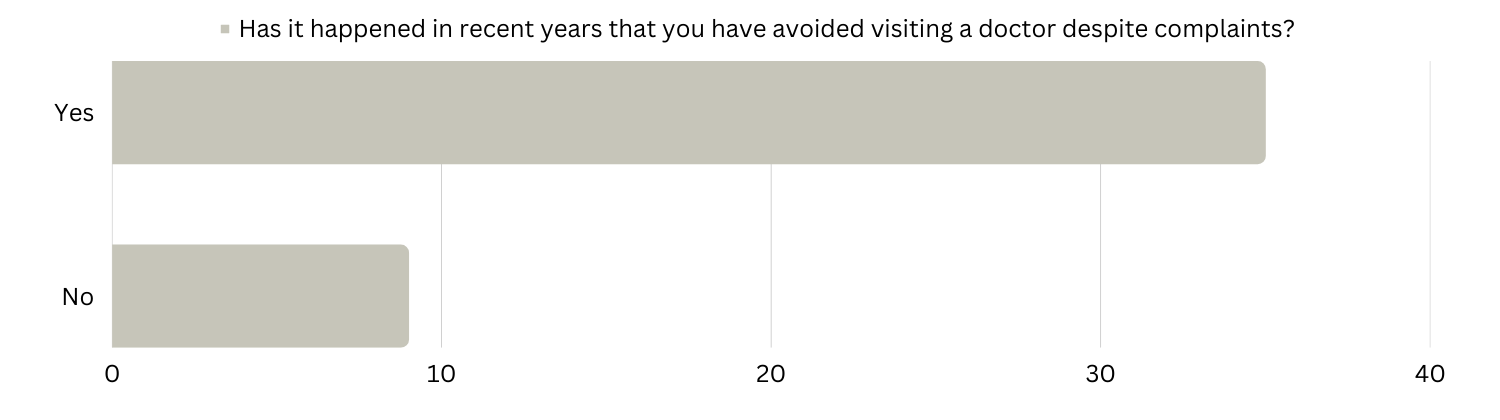
\includegraphics[scale=0.3]{avoidingDoctorYesNo.png}
	\caption[Survey Question]{Survey Question - Avoiding to visit the doctor}
\end{figure}
\noindent 
Another question in this survey asked respondents to list the justifications for delaying these doctor visits or the reasons they might consider forgoing a visit to the doctor.
Those reasons range from long waiting times, to difficulties scheduling an appointment. Figure 1.2 shows the mentioned distribution of the answers.
\begin{figure}[H]
	\centering
	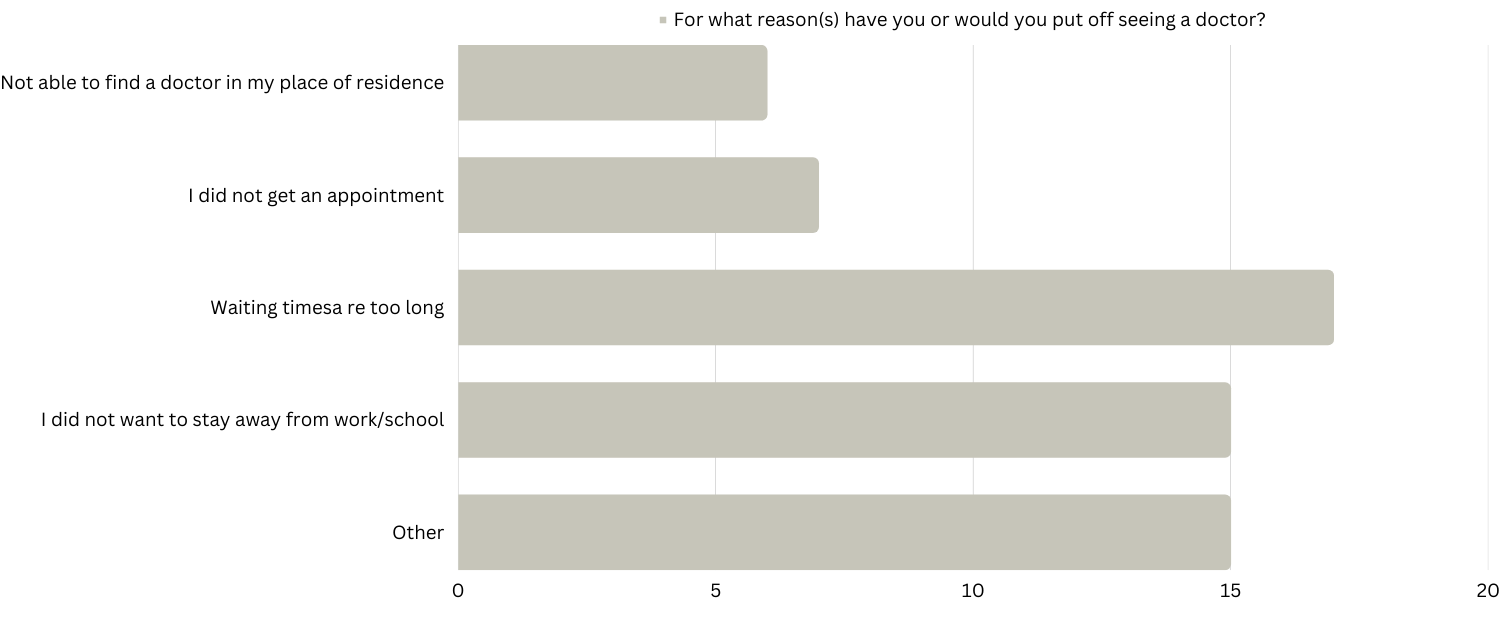
\includegraphics[scale=0.4]{reasonsPuttingOf.png}
	\caption[Survey Question]{Survey Question - Reasons of avoiding to visit the doctor}
\end{figure}
\noindent 
The answers given for the "other" option can be found in the appendix x.x.
\section{Motivation}
The mentioned problem imposes the question on how to address patients’ concerns while also relieving the burden on doctors. Digitalization provides a solution to this problem. Online consultation hours and appointment scheduling have recently helped relieve medical practices. Smartphones, in particular, are becoming an increasingly important part of our daily lives. The goal of this bachelor thesis is to provide a method for efficiently minimizing the aforementioned problems through the use of mobile applications. Such an application can provide advice to a worried user and help alleviate their fears.

\section{The Bachelor Thesis Goal}
The main focus of the work is on the conception of the application, the creation of a data structure and the determination of a calculation method for the diseases based on the symptoms given by the users, which results in a diagnosis. This diagnosis is made after successful data gathering regarding the user's symptoms and a subsequent determination of the possible diseases. Another goal of the application is that the database can be expanded by doctors, whereby a verification possibility must be provided to ensure that the person trying to log in is, in fact, a doctor. They should be provided with the possibility to add either disease-related data or pieces of advice regarding diseases and illnesses for users. 

\chapter{Related Works}
This chapter provides an overview of a selection of mobile applications that are comparable to the one in this work.

\section{Mobile Applications}
\subsubsection{ADA} 
\textbf{ADA} is the most popular symptom detection smartphone application. According to their own statements, their number of users is currently around 12 million, while 28 million symptom analyzes have already been completed.[ada website] The application is available free in the PlayStore and also in the Apple-Store. Disease detection in the ADA application is based on artificial intelligence developed by medical professionals of the ADA team. The user has the option of providing personal data in their user profile, such as allergies and medication intake. A symptom analysis starts by asking the user what their worst symptom is at the moment. Based on the user's answer, the AI searches its medical lexicon for this symptom and asks a symptom-specific question. An example of this would be to ask the user if he had enough water today, for the symptom headache. ADA uses a specially developed reasoning technology to assign symptoms. For this purpose, each symptom and each disease was assigned a common probability, which makes it possible to calculate the overall probability of the disease for the specific symptom analysis.[ada faq] After the successful diagnosis, the user has the option of downloading the diagnosis in PDF format, while they are also saved internally. The ADA application also makes its collection of knowledge available to users in the form of a disease dictonary. ADA also offers an API, which enables healthcare organizations to integrate the AI chat bot into their own application with the help of platform-specific SDKs. [api forum und faq]

\subsubsection{Diagnosis App} 
The \textbf{Diagnosis App} is another currently available application. It was created using the computer language C\# and the Unity platform. Here, the user has the option to select from a list of disease specifications, including those for diabetes test, thrombosis, depression, hair loss, headache, and gastrointestinal infection. During the survey procedure, a doctor's interview is simulated, where the user is prompted with questions after choosing one of these categories, similar to the ADA application. The most likely condition is then diagnosed based on the patient's responses, and various treatment choices are provided. The application was made specifically for people without medical experience and was created by German doctors and medical IT experts. According to the developers, an algorithm that accesses a medical database produces the diagnosis. Sadly, nothing more can be found out about the algorithm itself and how it works. 

\subsubsection{Other Solutions}
In addition to ADA and the Diagnosis App, other applications for symptom detection are available in the Playstore. However, these are nowhere near as accurate as those mentioned. Some of these applications are also only intended as reference book for symptoms and diseases, without a disease determination. In addition to mobile applications, there are also some web applications and websites available. However, this will not be discussed further in this work, since only mobile applications are dealt with here.

\section{Differentiation from other Systems}
In contrast to both of the applications mentioned, the knowledge base of the system should be able to be expanded by doctors who are not part of the development team. Similar to the Diagnosis App, the application presented in this work will not request any personally identifiable information from users. An expection is the case, when users wish to identify themselves as doctors. Unlike ADA, the diagnoses are not generated using AI, but are calculated by an algorithm. As already mentioned, the calculation process of the Diagnosis app cannot be determined and therefore no differentiation can be made from this application. With a realistic view, it can be said that this application cannot work as accurately as an artificial intelligence, that has been trained since 2011.  The aim of this work should not be to replace ADA as the market leader, not the Diagnosis App, but to describe the possible conception and implementation of such an application, while also comparing different calculation possibilities of the possible diseases, based on the user symptoms.




